\documentclass[10pt]{article}
\usepackage{fullpage}
\usepackage{amsmath,amsfonts,amssymb}
\usepackage{cite}
\usepackage{hyperref}
\usepackage{alltt}
\usepackage{graphicx}
\title{Assignment 1: Problem 1}
\author{Ernesto Rodriguez}

\begin{document}

\Huge{\bf Genetic Programming - Practical Assignment Part 1\\[1cm]}
\large{\bf Ernesto Rodriguez\\[0.5cm]}
\large{Student Id: 4083369}\\
\line(1,0){520}\\ \\

\section{Description of the Program}

The program provides a generic way to specify how selection, mutation, crossover and fitness measuring is done so the same routines can be used to evaluate a problem specified as a Genetic programming problem. The algebraic data type \verb+Env+ is used to provide such specification and is defined as follows:

\begin{alltt}

data Env (m :: * -> *) a where
  Env :: (MonadRandom m, I.MonadRandom m) => \{
    crossover :: [Vector a] -> m [Vector a],
    mutate :: Vector a -> m (Vector a),
    tournament :: forall x . Vector x -> m [Vector x],
    fitness :: (Vector a) -> Double,
    selOperation :: m Operation,
    target :: Vector a                 
  \} -> Env m a

\end{alltt}

The first component of env is the type parameter \verb+m+ which is simply a monad that allows the generation of pseudo-random values inside it. In most cases the IO Monad is used, but other monads can be considered, especially if the user wishes to run the algorithm inside a pure monad, like the State Monad, so the results are reproducible. 

The second component is a Haskell record denoted by \verb+Env+. This record contains the following fields:

\begin{itemize}
\item \verb+corssover+: The crossover operator. Given a selection of Vectors from the population, this function is responsible to combine them and produce the children. The function is allowed to use random computations.
\item \verb+mutate+: The mutate operator. When provided with a Vector, this operator is responsible to apply a random mutation to this vector. The main difference between the \verb+crossover+ \verb+mutate+ operators is that the \verb+crossover+ operator is allowed to see all the selected members.
\item \verb+tournament+: This function is responsible to select members from the population that will be mutated or mixed with crossover. The function is a polymorphic function that given a vector of elements, must return several vectors of containing elements of the input parameter. From each of the returned vectors, the strongest member is selected using the fitness function. In other words, every vector in the returned list will be reduced to the single strongest element and after the list is reduced, it will be passed to the \verb+crossover+ or \verb+mutate+ operators.
\item \verb+fitness+: The Fitness function which given a vector, calculates a real number that represents the fitness of that vector. This is the function that will be used to swap members from the population and select members from a tournament selection.
\item \verb+selOperation+: This function is responsible for deciding whether the \verb+crossover+ or \verb+mutate+ operator will be used. It is called every time candidates from the population are chosen and is allowed to use random operations to make a decision.
\item \verb+target+: The goal of the algorithm. If that element is produced, the algorithm will be stopped.
\end{itemize} 

The program also provides some implementations of these parameters. They are the following:

\subsection{Crossover Implementations} 

\verb+uniformCrossover+: It takes as an argument the probability of choosing one bit from the first parent against choosing the bit from the second parent. It then will return a uniform crossover operator for the given probability.
\\\\
\verb+twoPointCrossoverAll+: This crossover operator splits the child vector into two sections and fills one section with the values from the first parent and the second section with values of the other parent. The sections are selected as follows, first two numbers are produced:
\[
x_0 \sim \mathcal{U}(0,l)
\]
\[
x_n' \sim \mathcal{N}(x_0 + l/2,l/s)
\]
\[
x_n = \left\{
    \begin{array}{l l}
    x_0 & \quad \text{if $x_n' < x_0$}\\
    x_0+l-1 & \quad \text{if $x_n' \geq x_0 + l$}\\
    x_n' & \quad \text{otherwise}
    \end{array} \right.
\]
where,
\begin{itemize}
\item $l$ is the the size of the bits vector.
\item $s$ is the deviation parameter of the function
\end{itemize}

Then given the parent vectors $v_a$ $v_b$, the ith element of the result vector $v_{res}$ is selected as follows:
\[ v_{res}[i] = \left\{ 
  \begin{array}{l l}
    v_a[i] & \quad \text{if $i \in \{x \mod{l}\ |\ x = x_0 .. x_n \}$}\\
    -(n+1)/2 & \quad \text{otherwise}
  \end{array} \right.
\]

The intuition here is selecting an index ($x_0$) at random and then selecting an offset from the index ($x_n$) which will be on average half the length of the vector but distributed normally across multiple possible lengths. Then the selected range is assigned values from one parent and the remainder is assigned values from the other parent.
\\\\
\verb+randomizedTwoPointCrossover+: This operator operates the same way as the \verb+twoPointCrossoverAll+ except that the \verb+mutate+ operator described above is applied to each of the parents before doing the crossover. In fact it is defined as:
\begin{alltt}
 randomizedTwoPointCroosver\ =\ twoPointCrossoverAll s . mapM mutateDefault
\end{alltt}

As it can be observed, it is simply the function composition of mutating all the input parents and then applying the standard two point crossover. This operator was introduced with the hope that it would better preserve diversity than using the mutate and crossover operators independently.

\subsection{Mutate Implementations}

\verb+mutateDefault+: This function flips the value of $n$ random bits in a vector with probability $1/n$.

\subsection{Fitness Implementations}

\verb+trapFunction+: Implementation of the trap fitness function. It takes as arguments a value for $k$ and $s$.
\\\\
\verb+ungroupedTrapFunction+: It behaves exactly the same as the trap function, but it takes an additional mapping $m$ as argument, which is a vector where the value of each index indicates the index of that value in the mapped vector. Formally it is:
\[
v_m[i]\ =\ v_{in}[m[i]]
\]
where,
\begin{itemize}
  \item i indicates the ith index
  \item $v_m$ is the new vector for which the trap function will be applied
  \item $m$ is the vector with mappings
  \item $v_{in}$ is the input vector
\end{itemize}

\subsection{Tournament Implementations}

\verb+tournamentN+: This function performs tournament selection. The fist argument provided is the number of tournament selections to be done and the second argument indicates the tournament size. Normal values for this function would be 2 for number of selections and 2 for tournament size which will select two elements using tournaments of size 2.

\subsection{Operator Selection}
\verb+selFun+: This function takes as an argument the probability of selecting the crossover operator encoded as a rational number.
\\\\
\verb+defSel+: This function selects the \verb+mutate+ and \verb+croosover+ operators with equal probability.

\subsection{Flow}

There exists several functions responsible for evolving a population under the conditions of a particular environment until a global optimal is found or no improvement happens for a long time. The most important functions outlined below.
\\\\
\verb+runExperiment+: I takes an environment and a generation size as a parameter. It then proceeds to evolve the generation with the operators and fitness function provided with the environment. It uses the function \verb+nextGenerations+ to produce the subsequent generations.
\\\\
\verb+nextGenerations+: This function produces new generations until the global optimal solution is produced or no improvement happens in 10 times the population size. This function is a wrapper for the \verb+nextGenerationsS+ which does the actual work inside the State Monad to allow a more optimized implementation using tail recursion.
\\\\
\verb+performOperation+: Function responsible for producing a new member for the population. It is provided with the environment, an operator and a population. It then proceeds to select members from the population using the tournament function and applies the operator to those elements. It then measures the fitness of the resulting element and adds it to the population if it is fit enough.

\subsection{Generations}

For all bookkeeping concerning the administration of generations, the specialized \verb+Generation+ data type is used. This data type contains a vector with all members of the population along with their fitness. This avoids recomputing the fitness whenever members of the population are being compared. Another optimization is that the structure keeps track of the strongest and weakest members of the population. This reduces the computational time required to determine whether a solution will be allowed to enter the population. Once a new solution is added to the population, the strongest and weakest members can be found in linear time.

\section{Description of the Experiment}

The objective of this experiment was to test genetic algorithms on several different functions and study their behavior using different parameters for the algorithms. The functions that were tested are:

\begin{itemize}
\item Uniformly Scaled Counting Ones Function
\item Linearly Scaled Counting Ones Function
\item Non-Deceptive Trap Function ($k=4,\ d=2.5$)
\item Deceptive Trap Function ($k=4,\ d=1$)
\item Randomized Deceptive Trap Function
\end{itemize}

To solve these functions, three crossover operators and one mutate operators were used. The crossover operators were: \verb+uniformCrossover+, \verb+twoPointCrossover+ and \verb+randomizedTwoPointCrossover+. The mutate operators were: \verb+mutateDefault+. 

Two different methods for sampling the population were used, namely one member tournament and two member tournament. In the first case a single element was chosen at random and in the second case, two elements were chosen at random and the fittest one was chosen as the sample.

Three operator selection criteria were used: Choosing mutate with 100\% probability, choosing mutate and crossover each with 50\% probability and choosing crossover with 100\% probability. 

All combinations of the above parameters were tested with populations of size 30 to 450 in population increments of 30 members. An experiment with a particular selection of parameters and population size was repeated 30 times and the results were averaged.
\pagebreak
\section{Results and Discussion}

\subsection{Uniformly Scaled Counting Ones Function}

\begin{figure}[h!]
  \centering
    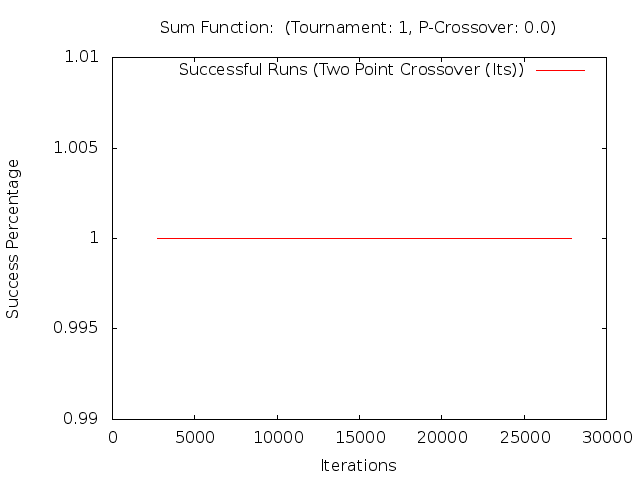
\includegraphics[height=170px]{img/SumFunctionRandomIters.png}
    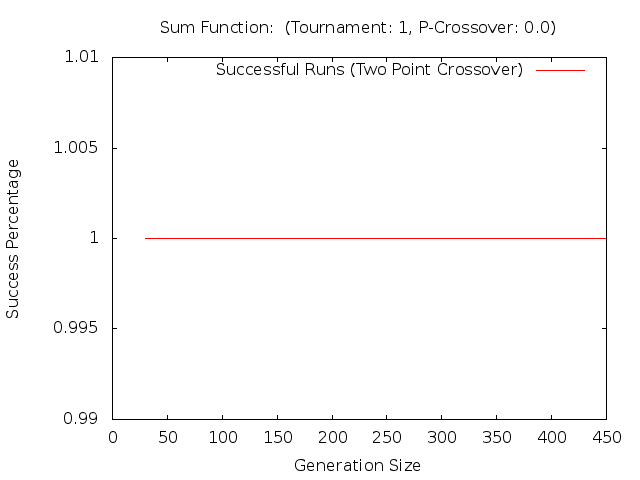
\includegraphics[height=170px]{img/SumFunctionRandomGens.png}
    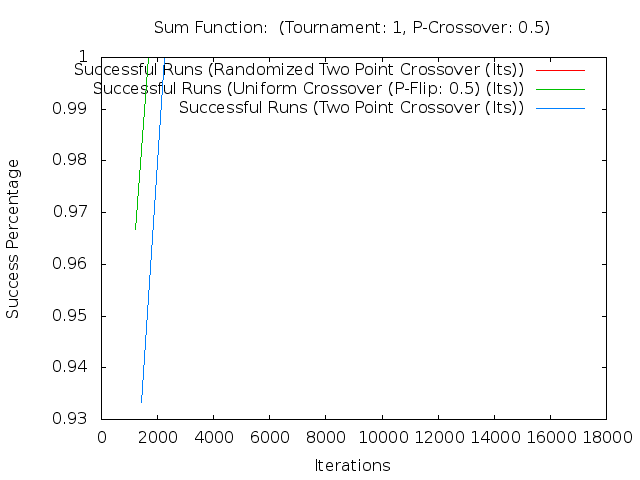
\includegraphics[height=170px]{img/SumFunctionBothIters.png}
    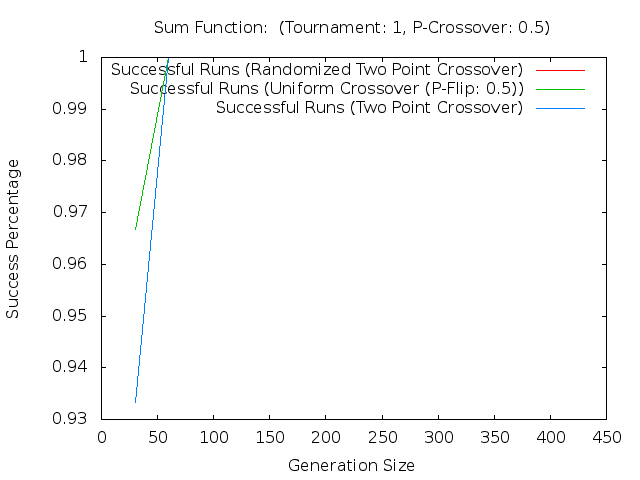
\includegraphics[height=170px]{img/SumFunctionBothGens.png}
    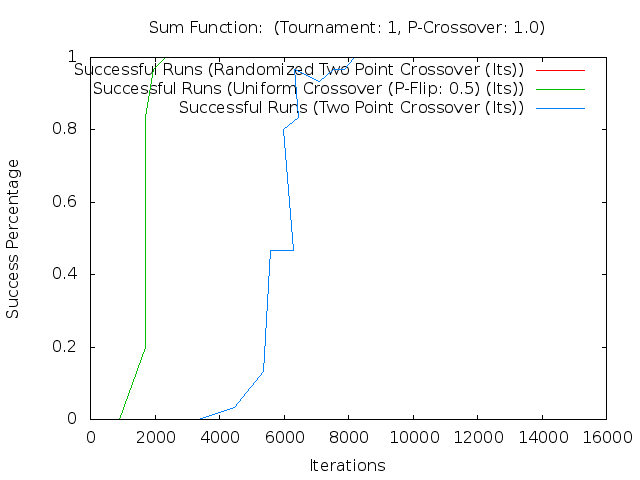
\includegraphics[height=170px]{img/SumFunctionCrossoverIters.png}
    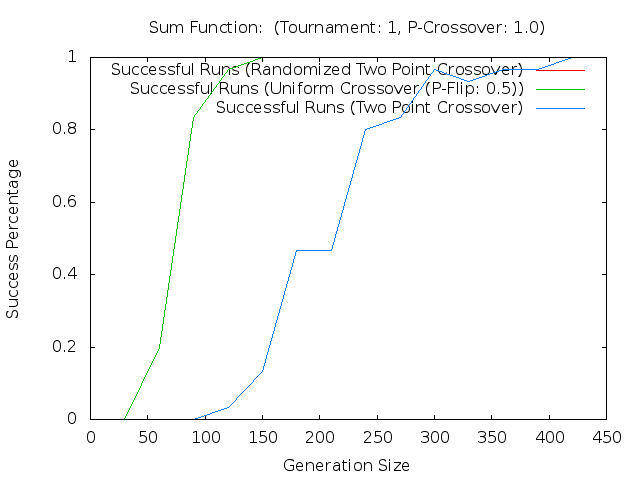
\includegraphics[height=170px]{img/SumFunctionCrossoverGens.png}
    \caption{Performance for the Uniformly Scaled Counting Ones Function}
\end{figure}

The uniformly scaled counting ones function is a very simple function. As expected, all methods were able to find the global maximum with generations of sizes as small as 30. Except for the case of the randomized two point crossover operator, the crossover operator did not provide a significant advantage in number of iterations required to find a solution. For this case, the randomized two point crossover operator was the one that could find solutions with least number of iterations.

\pagebreak
\subsection{Linearly Scaled Counting Ones Function}

\begin{figure}[h!]
  \centering
    \includegraphics[height=170px]{img/ScaledSumFunctionRandomIters.png}
    \includegraphics[height=170px]{img/ScaledSumFunctionRandomGens.png}
    \includegraphics[height=170px]{img/ScaledSumFunctionBothIters.png}
    \includegraphics[height=170px]{img/ScaledSumFunctionBothGens.png}
    \includegraphics[height=170px]{img/ScaledSumFunctionCrossoverIters.png}
    \includegraphics[height=170px]{img/ScaledSumFunctionCrossoverGens.png}
    \caption{Performance for the Linearly Scaled Counting Ones Function}
\end{figure}

In the case of linearly scaled counting ones function, random mutation is the clear winner. Even when small generations were used, it could quickly find the optimal solution. The important aspect when it comes to random mutation is that enough mutations are attempted before giving up (after 10 times generation size repetitions). This way an improvement can easily follow since it will take place once a 0 is flipped into a one which is something likely to happen if the probability of flipping few bits is high (if many bits are flipped, the chances that all of them will be one is low once again).

The best operator was clearly the randomized two point crossover. It was the only operator that could find the optimal solution by itself. It is evident that for this problem, random mutation is important to reach a solution. The disappointing part is that there appears to be no advantage using a crossover operator to solve this problem. Except for the randomized two point crossover operator, the presence of the operator only seemed to impose more iterations to reach the solution.
\pagebreak
\subsection{Trap Function}

\begin{figure}[h!]
  \centering
    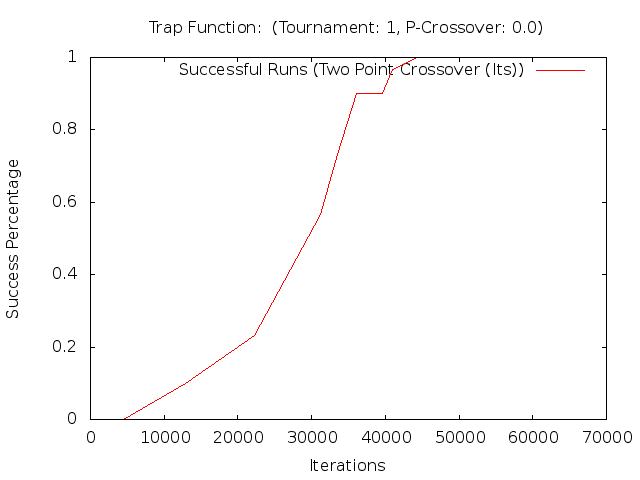
\includegraphics[height=170px]{img/TrapFunctionRandomIters.png}
    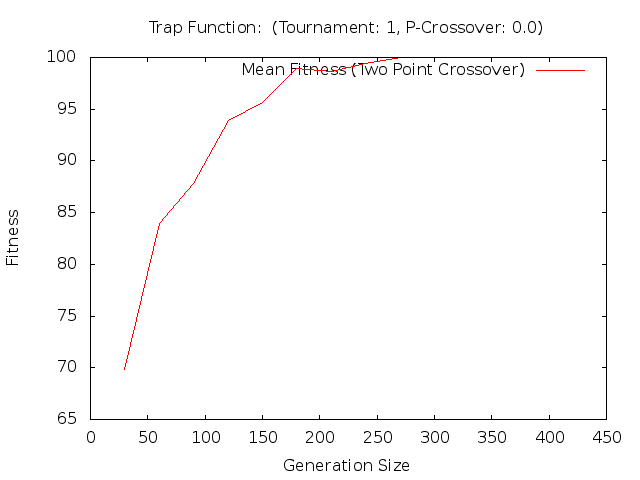
\includegraphics[height=170px]{img/TrapFunctionRandomGens.png}
    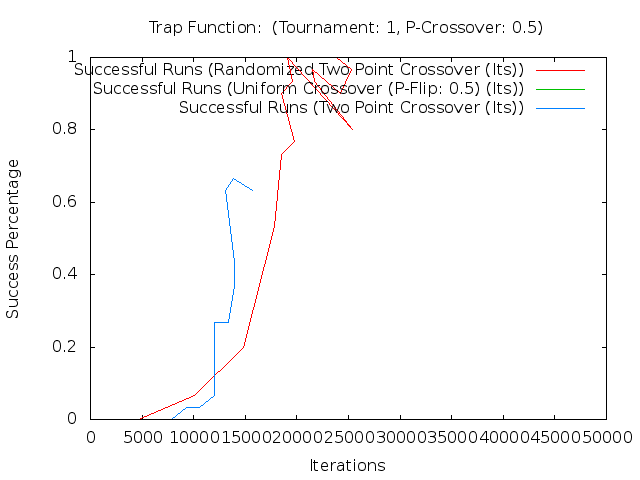
\includegraphics[height=170px]{img/TrapFunctionBothIters.png}
    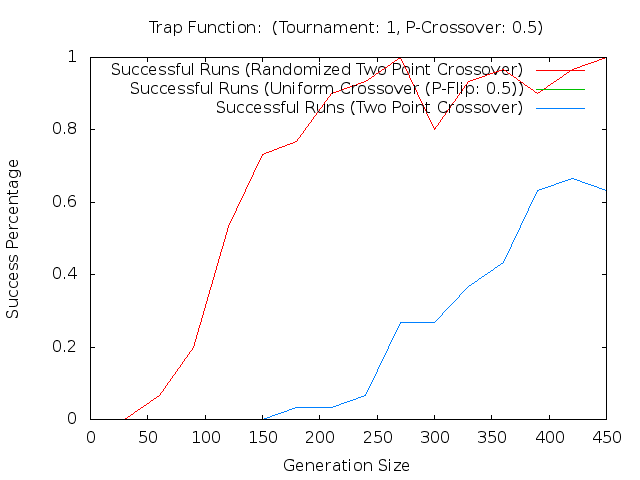
\includegraphics[height=170px]{img/TrapFunctionBothGens.png}
    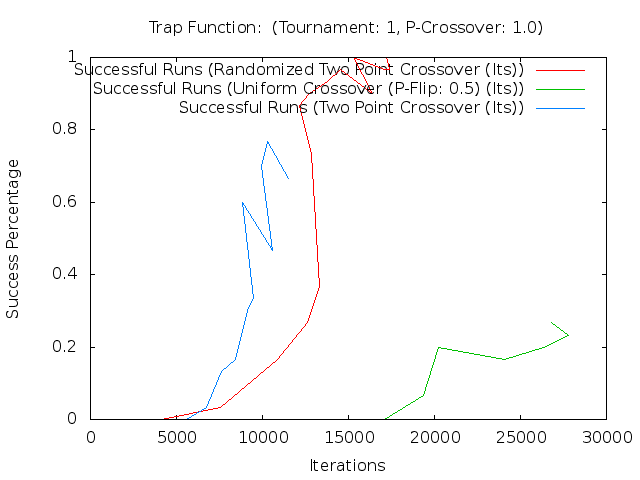
\includegraphics[height=170px]{img/TrapFunctionCrossoverIters.png}
    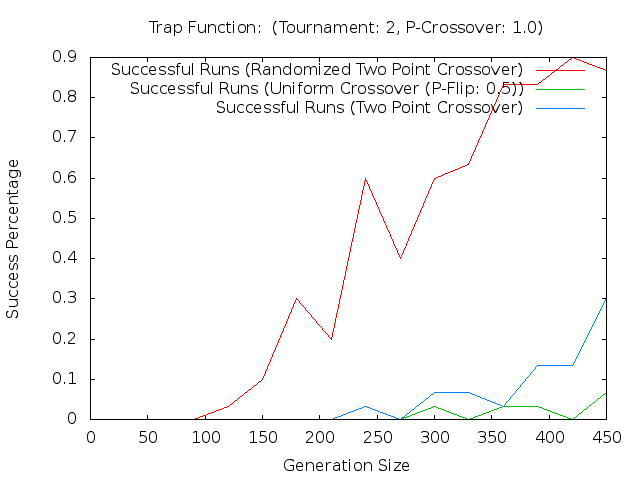
\includegraphics[height=170px]{img/TrapFunctionCrossoverGens.png}
    \caption[Performance for the Trap Functions]{Performance for the Trap Functions}
\end{figure}

For the Trap Function, solely random mutation produced the best performance. With generation sizes of around 300 members and 50,000 iterations it could find the global optimum for all the runs. For this function, one can expect random mutation to work well with big enough populations since any zero that gets flipped into a one will result in an improvement. Since the stop criteria required no improvement a significant amount of iterations without improvement (4,000 when generation is 400) it was very likely that an improvement occurred in these conditions.

The added value for this case for crossover is the faster convergence speed. The randomized two point crossover operator could find global optimums by itself with about 15,000 iterations and generations of 300 members. This is a considerable improvement on use of resources. This function also suggests that combining mutation and crossover in a single operator has an added extra value since the randomized two point crossover operator had better performance than combining mutation and two point crossover each with 1/2 probability. The uniform crossover operator did not perform well at this task. Especially since it required much more runs and produced no improvement over other methods.
\pagebreak
\subsection{Deceptive Trap Function}

\begin{figure}[h!]
  \centering
    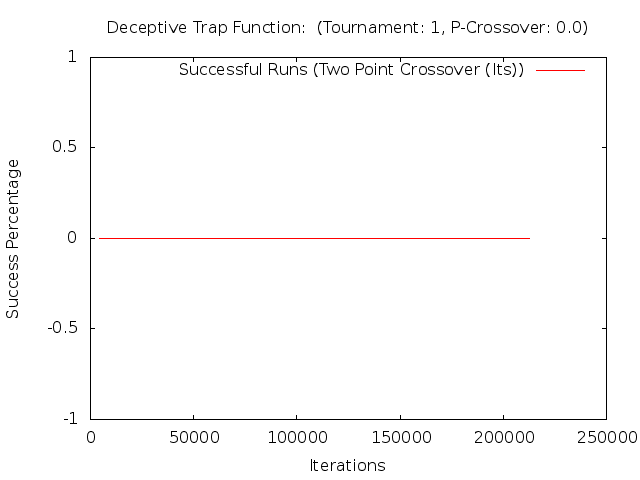
\includegraphics[height=170px]{img/DeceptiveTrapFunctionRandomIters.png}
    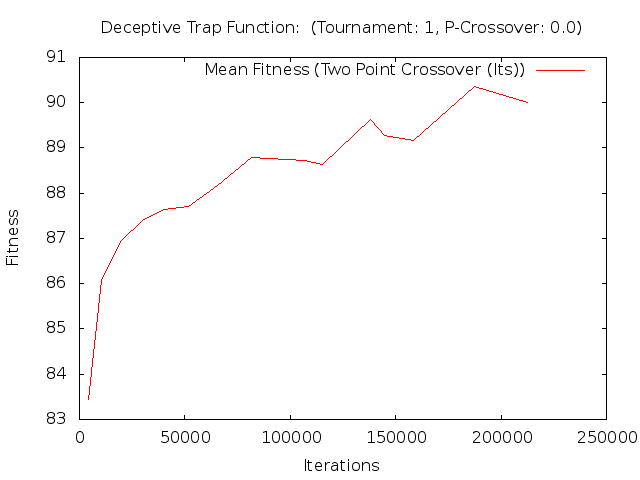
\includegraphics[height=170px]{img/DeceptiveTrapFunctionRandomFitness.png}
    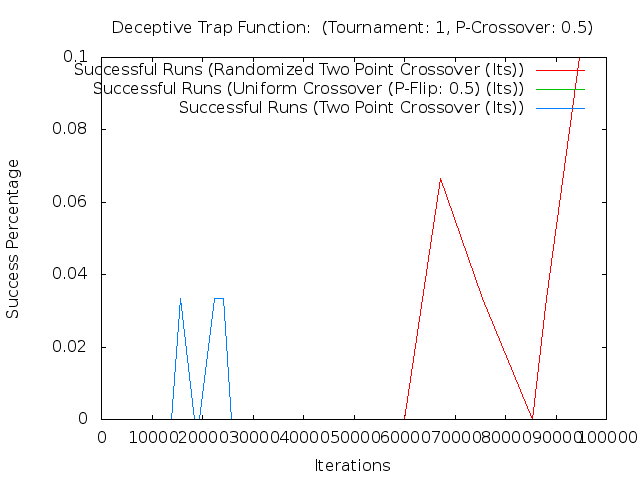
\includegraphics[height=170px]{img/DeceptiveTrapFunctionBothIters.png}
    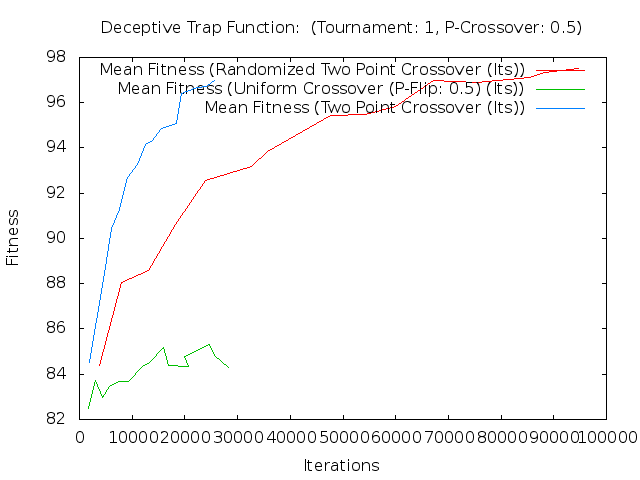
\includegraphics[height=170px]{img/DeceptiveTrapFunctionBothFitness.png}
    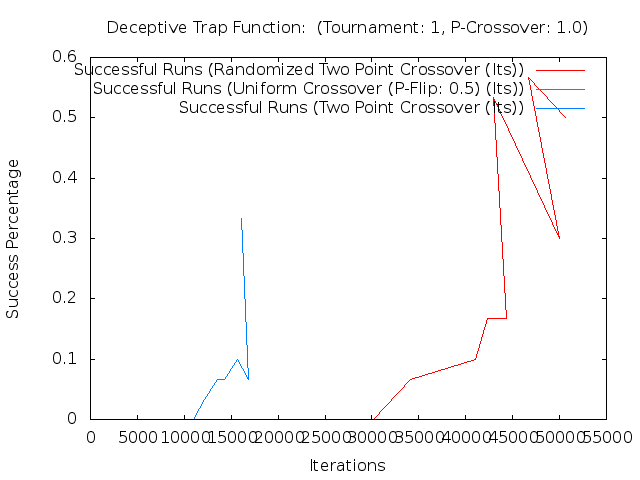
\includegraphics[height=170px]{img/DeceptiveTrapFunctionCrossoverIters.png}
    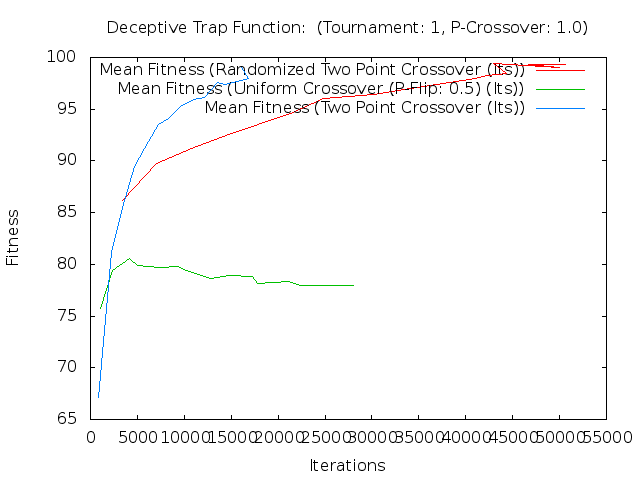
\includegraphics[height=170px]{img/DeceptiveTrapFunctionCrossoverFitness.png}
    \caption[Performance for the Trap Functions]{Performance for the Trap Functions}
\end{figure}

For the deceptive trap function, complete randomness also produced solutions with very strong fitness after many iterations. An average 90 for the maximum fitness was obtained with this approach with 200,000 iterations. Nevertheless, this case was favorable for algorithms that used crossover. The results were specially favorable when using tournament 1 selection and 1.0 crossover probability. For these cases, the two point crossover and randomized two point crossover operators managed to find the global optimal very reliably once the generation size was over 300 elements with less than 50,000 iterations showing very superior results to those using only randomness. Another surprising result is that results were better when mutation and crossover were used with equal probability. 

Although mutation is an important element that allows a more widespread exploration of solutions, the two point crossover by itself could produce good solutions in less iterations than the mutate operator. This could stem from the fact that the initial population is generated randomly, so this still provides the two point crossover with some randomness, especially if the population is big so a lot of diversity is preserved. Nevertheless, random mutation is important and this is made evident by the fact that the two point crossover performed better when mutation probability was 50\% and because the randomized crossover operator always did better. An interesting remark is that the randomized two point crossover operator always did better than the two point crossover operator. This suggests that there might be an added extra value in combining crossover and mutation in a single operator.

\pagebreak
\subsection{Randomized Deceptive Trap Function}

\begin{figure}[h!]
  \centering
    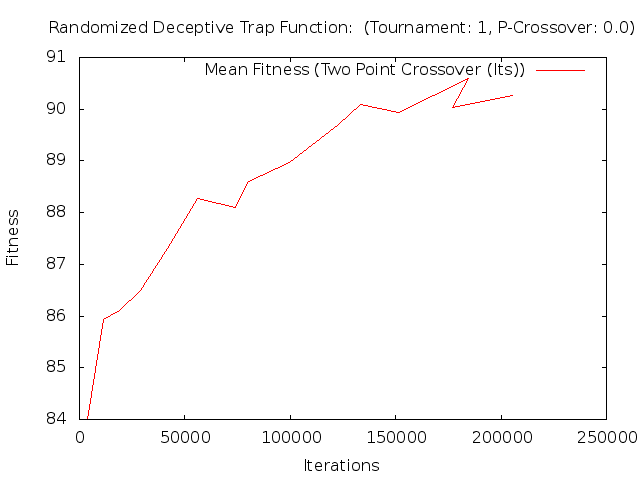
\includegraphics[height=170px]{img/RandomizedDeceptiveTrapFunctionRandomIters.png}
    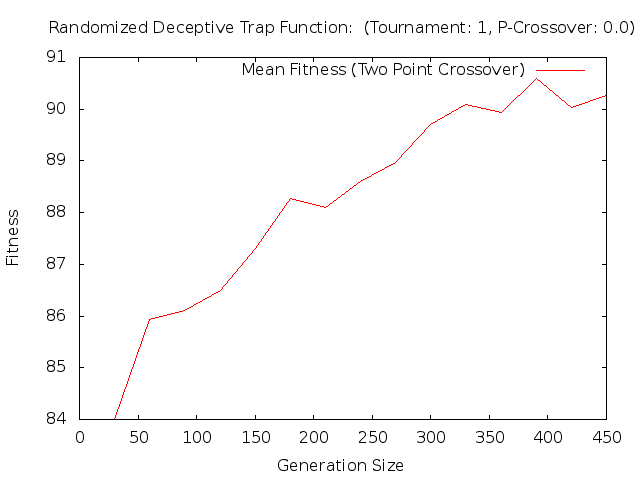
\includegraphics[height=170px]{img/RandomizedDeceptiveTrapFunctionRandomGens.png}
    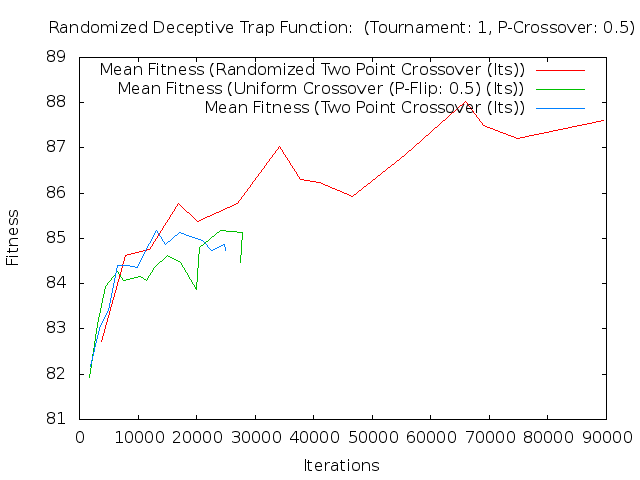
\includegraphics[height=170px]{img/RandomizedDeceptiveTrapFunctionBothIters.png}
    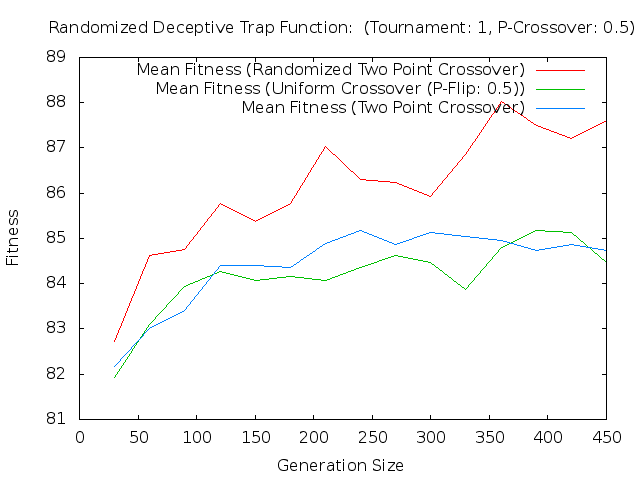
\includegraphics[height=170px]{img/RandomizedDeceptiveTrapFunctionBothGens.png}
    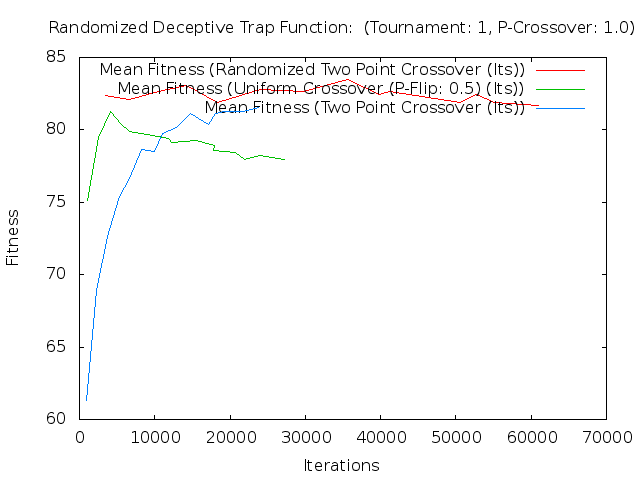
\includegraphics[height=170px]{img/RandomizedDeceptiveTrapFunctionCrossoverIters.png}
    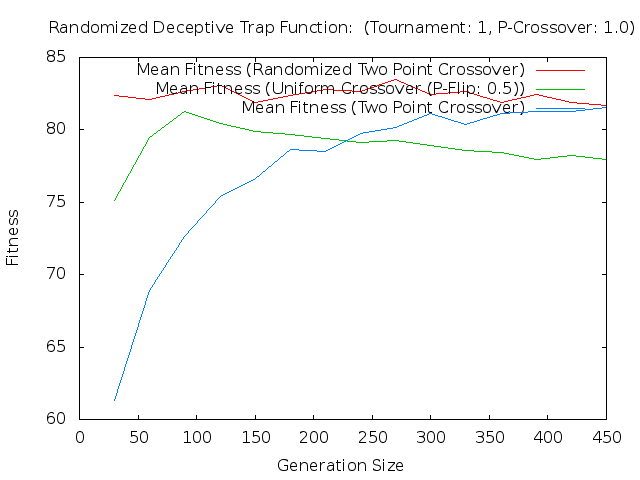
\includegraphics[height=170px]{img/RandomizedDeceptiveTrapFunctionCrossoverGens.png}
    \caption[Performance for the Trap Functions]{Performance for the Trap Functions}
\end{figure}

In the case of the Randomized Deceptive Trap Function, the operator that found the best solutions was simply random mutation. The runs that used the crossover operator usually had difficulties preserving the population diversity.

Observing the evolution of the population in some informal experiments, the case usually was that after reaching certain fitness value, the entire population began converging to a local optimal value which eventually became the entire population. It appeared to be the case that no matter what element was produced by crossover, it would only be accepted if it was the already found local maximum value.

To work around the situation, several approaches were considered. First, running the experiment with a higher probability of mutation over crossover was performed. The performance was usually better but the disappointing part was that the best results were still occurred when no crossover was used.

A final effort to increase diversity was combining the two-point crossover with mutation. In this case, each of the parents was mutated before applying the two point crossover. As it can be seen in the benchmarks, this method performed better than the other crossover operators and yielded comparable results to random mutation with much less iterations.

It can be hypothesized from the results that by random mutation it is very unlikely that an improvement will happen for this function. Therefore, the crossover operator quickly filled the population with a sub-optimal solution and it was very difficult to keep diversity because the solutions resulting from random mutations were usually weaker. The combination of crossover with mutation in a single operator seemed to allow more diversity to occur. No hard statements can be made about why it is so, but that is the way it happens in nature. Mutation and gene transfer occurs as a single operation.

\section{Conclusions}

For the simple problems considered (linearly scaled counting ones function and linearly scaled counting ones function), random mutation was the key factor to solve the problems. Both of these problems had a single global maximum value and any mutation that flipped one or more zeros to one would be considered an improvement. The crossover operators considered here were not suited for these problems since no performance advantage was gained by using them.

The Trap Function was still no challenge for random mutation but there were significant performance improvements with respect to the number of iterations required to solve the problem. When mutation was combined with two point crossover, the solution was found in half the number of iterations. This problem shows the importance of choosing a good crossover operator since the uniform crossover operator was still not capable of finding the global optimal solution reliably.

The deceptive trap function posed a bigger challenge since random mutation could not find solutions by itself. The best performance was achieved when using the two point crossover by itself, especially the randomized two point crossover. This seems to suggest there is an added value combining mutation and crossover into a single operation. It was probably helpful to use the two point crossover operator since it would promote continuous strings of ones to evolve quickly.

Once the bits were no longer adjacent, the deceptive trap function became much more difficult. For random mutation, it makes no difference to change the order of bits for the deceptive trap function since it doesn't exploit any topological properties of the bit string. Nevertheless, this function could not be solved by any combination considered here hence the average fitness was plotted instead of the success rate since it was zero for all cases. The performance benchmarks were favorable for the cases that exclusively used random mutation. In some occasions, the randomized two point crossover operation could achieve better performance with less iterations but it wasn't the case in general.

The experiment could be changed to further explore thees problems. One improvement that can be considered is replacing more members of the population with each iteration. Currently several members are considered to enter the next generation but only the fittest one is taken. Taking all members that are still stronger than the weakest player could at least improve the number of iterations required to find a solution. 

\end{document}
